%----------------------------------------------------------------------------
%----------------------------------------------------------------------------
The Stanford Research Systems SR250 Gated Integrator was used to temporally sample, amplify, and average the pulsed signal from the RF receivers. Even with a high pass filter between the photodiode and the receiver, the output from the receiver above 150 MHz was buried in the noise. The boxcar averager was required to retrieve the signal from the usable range of each receiver. When the receiver's center frequency is tuned down to about 130 MHz, a significant signal can be seen from the receiver ($\sim$15 mV). This signal is used to place the boxcar gate. See Fig. \ref{gate}
%----------------------------------------------------------------------------
%----------------------------------------------------------------------------
%----------------------------------------------------------------------------
\begin{figure}
\begin{center}
\leavevmode
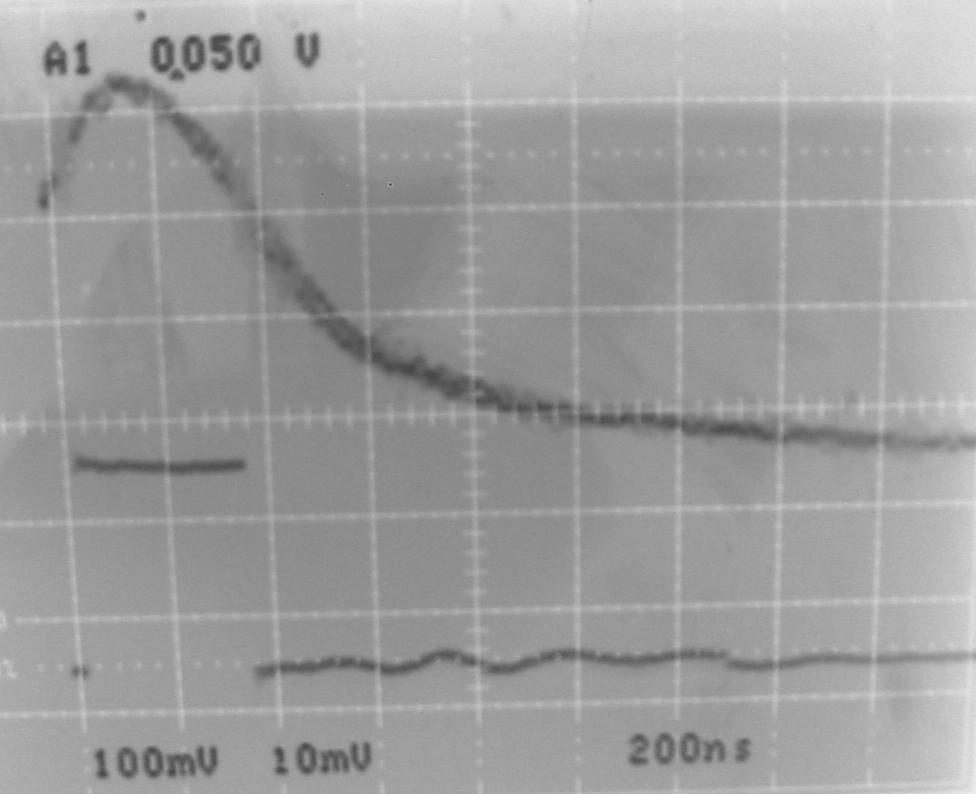
\includegraphics[width=4in]
{gate/gate.png}\\
\end{center}
\caption[Boxcar gate placement for RF beat measurement]{Boxcar gate placement for RF beat measurement. Channel one is the gate (lower trace, 100 mV/div), channel two is the receiver output (upper trace, 10 mV/div). This picture was taken with the receiver tuned to 50 MHz before we had the high pass filter, hence the large signal. Once the high pass filter was in place this ``DC'' signal was only $\sim$15 mV. This signal was only used to place the gate - data was not taken this close to DC.}
\label{gate}
\end{figure} 
%----------------------------------------------------------------------------

%----------------------------------------------------------------------------
for a view of the oscilloscope during gate alignment. Once the gate is placed, appropriate gate widths, sensitivity settings, and sample numbers are selected. The boxcar gate is not temporally scanned in this experiment.

%----------------------------------------------------------------------------
%----------------------------------------------------------------------------
